\documentclass[10pt]{article}
\usepackage{graphicx}
\usepackage{float}

\begin{document}
\title{Super Duper Joke Attack()}
\author{Paul D. Camarata}
\date{1 August 2018}

\maketitle
\pagebreak
\begin{abstract}
The most exciting phrase to hear in science, the one that heralds new discoveries, is not 'Eureka!' (I've found it!), but 'That's funny...' -Isaac Asimov.
\end{abstract}

\section{Introduction}
The purpose of this exploitation project was to gain a better understanding of how to recognize and take advantage of a buffer overflow vulnerability.  It is broken apart into two sections.  The primary section is dedicated to identifying and exploiting a very basic overflow vulnerability.  The second section is the extra credit portion.  Based on the samples given throughout the week, and made available to us via a web tutorial, the actual execution was extremely simple.  The overall objective is to capture the flag, “Nice job! Teacher, give this student an A.” located in the binary.  

\section{Part I: The Assignment}
Part I, the assignment portion, presented us with one, basic, file, tellMeAJoke.  The images included are here to reference the work that was done locally.  The assignment is broken apart into three logical sections.  First we will do a quick review of the file by itself, static analysis.  Secondly, we will beging executing and debugging the file, dynamic analysis.  

\subsection{Static Analysis: Pre-Debugger}
Figure 1 is a reference to running the 'file' command.  The goal here is to understand what we are working with, and in what architecture  a dynamic analysis will work.

\begin{figure}[H]
\centering
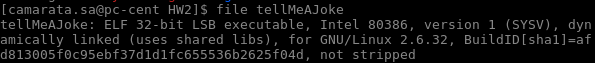
\includegraphics[scale=0.5]{./images/ss1.png}
\caption{file}
\label{fig:Code}
\end{figure}

Our target is the flag.  Since we know it is a string in the file, we will do a quick dump of the strings to see if there is any additional information we can infer.

\begin{figure}[H]
\centering
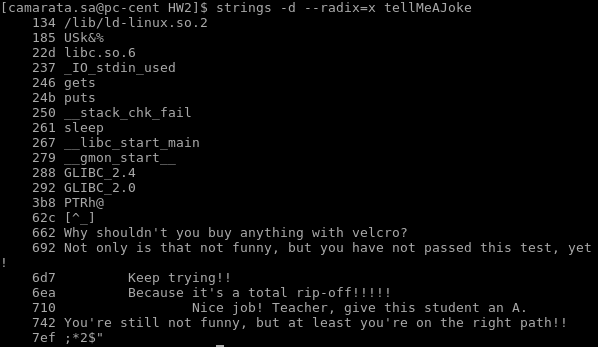
\includegraphics[scale=0.5]{./images/ss3.png}
\caption{strings}
\label{fig:Code}
\end{figure}

We can see that our flag does exist in the file and we can even see some additional strings that we might expect to find as we begin executing the file.

\subsection{Static Analysis: Debugger}
It is now time to fire up the debugger.  We are intentionally using gdb here vice any of the alternative debuggers.

\begin{figure}[H]
\centering
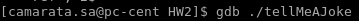
\includegraphics[scale=0.5]{./images/ss4.png}
\caption{gdb}
\label{fig:Code}
\end{figure}

First things first, we are going to set our assembly flavor.  We've only been practicing intel based architecture in class so that is what we will use.

\begin{figure}[H]
\centering
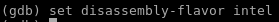
\includegraphics[scale=0.5]{./images/ss5.png}
\caption{flavor}
\label{fig:Code}
\end{figure}

We are going to assume that the program is a compiled C program and attempt to disassemble the main() function.  If this assumption was false, there would be some additional preamble that we would attempt here.

\begin{figure}[H]
\centering
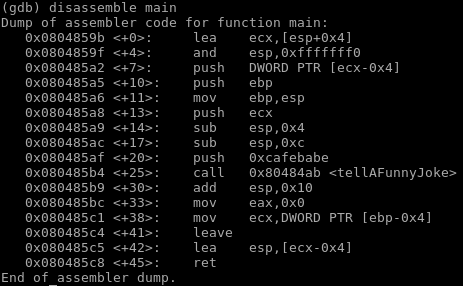
\includegraphics[scale=0.5]{./images/ss6.png}
\caption{disassemble main}
\label{fig:Code}
\end{figure}

There is very little of note here.  The only thing that points us in any direction is a call to another function called tellAFunnyJoke().  Now we disassemble this function.

\begin{figure}[H]
\centering
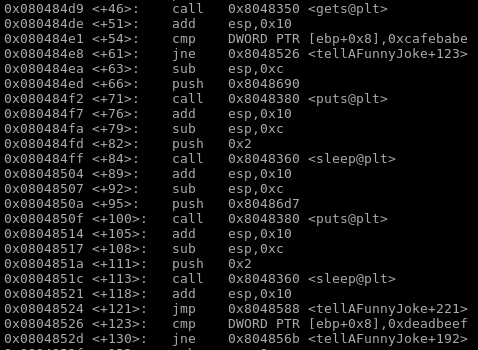
\includegraphics[scale=0.5]{./images/ss7.png}
\caption{disassemble tellAFunnyJoke}
\label{fig:Code}
\end{figure}

The output has been substantially truncated and only a relevant section is presented.  Basically here we see that there is a call for input and then two potential jumps (jne) based on compares (cmp) to a couple of hex values.  Based on the examples, these are the most likely locations for our flag to be found.  A quick examination of the jump locations will likely lead us to our string.  Our first goal is to examine these memory locations using gdb.

\begin{figure}[H]
\centering
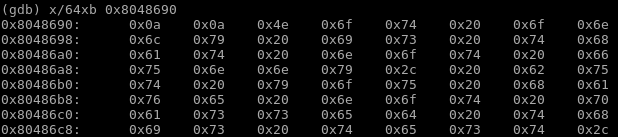
\includegraphics[scale=0.5]{./images/ss8.png}
\caption{x/64xb 0x8048690}
\label{fig:Code}
\end{figure}

If we were to present the hex value of 0xcafebabe to this compare, then we would print the information available at this location.  A quick hex to ascii conversion shows us that this location contains "Not only is that not funny, but you have not passed this test," which is not our desired flag.  Time to check out our second potential compare.

\begin{figure}[H]
\centering
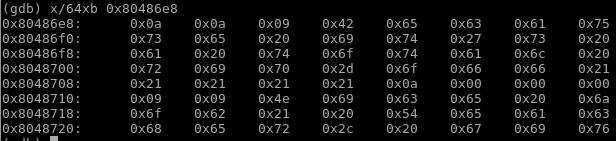
\includegraphics[scale=0.5]{./images/ss9.png}
\caption{x/64xb 0x8048690}
\label{fig:Code}
\end{figure}

Here we see what would potentially be output if we instead presented the hex value of 0xdeadbeef.  Doing another hex to ascii conversion, we are presented with "Because it's a total rip-off!!!!!" and "Nice job! Teacher, giv." Voila, we have found the desired location in memory to capture our flag.  The only thing left to do is to manipulate the program to get us there.

\subsection{Dynamic Analysis}
Since we downloaded this file from the internet, we will need to add the executable bit to make it runnable.

\begin{figure}[H]
\centering
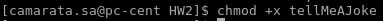
\includegraphics[scale=0.5]{./images/ss2.png}
\caption{chmod +x}
\label{fig:Code}
\end{figure}

We need to figure out how much data we can pump into the buffer and then how much we need to overflow to force the program to jump where we want.  First things first, we set out break point to examine the stack at the desired location.

\begin{figure}[H]
\centering
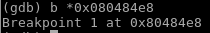
\includegraphics[scale=0.5]{./images/ss10.png}
\caption{b *0x080484e8}
\label{fig:Code}
\end{figure}

Here we are setting a break just after the first compare and before the jump.  History has shown us that the gets() call is overflowable.  Once we set our break point, it is time to execute our program.

\begin{figure}[H]
\centering
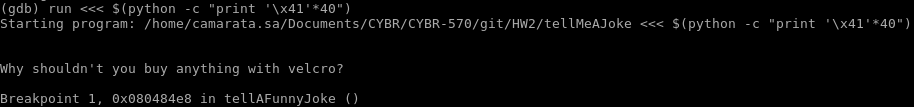
\includegraphics[scale=0.5]{./images/ss11.png}
\caption{run}
\label{fig:Code}
\end{figure}

Here we are executing the program and inserting 40 hex values of 0x41, or A in ascii.  The goal is to pad our stack to see how we are manipulating it easily.  The application runs until we hit our break point, and it is time to examine the stack.

\begin{figure}[H]
\centering
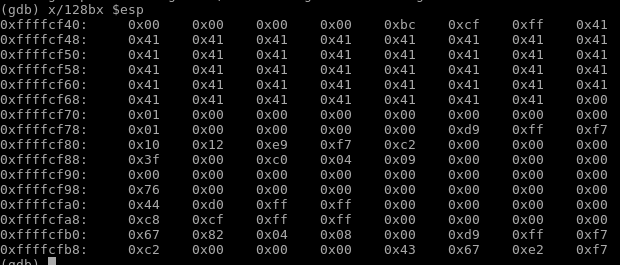
\includegraphics[scale=0.5]{./images/ss12.png}
\caption{stack}
\label{fig:Code}
\end{figure}

Here we are examining 128 bytes in hex of the stack.  We can easily see our inserted hex values.  The key thing to note here is that it starts at 0xffffcf47.  Now we need to see if there is any additional information in our registers of note.

\begin{figure}[H]
\centering
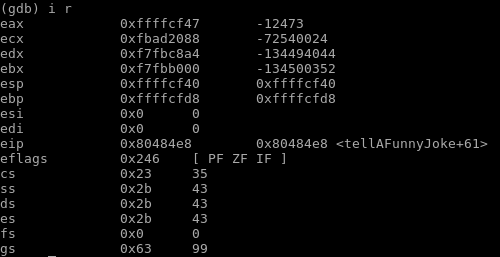
\includegraphics[scale=0.5]{./images/ss13.png}
\caption{registers}
\label{fig:Code}
\end{figure}

Specifically we are looking at the ebp register.  If you recall Figure 6, we see that it is comparing our static hex value 0xdeadbeef to what is contained in ebp + 0x08.  Our ebp is located at 0xffffcfd8 and is exactly 0x90 or 145 bytes away.  If we add the 8 additional bytes, then we are an even 153 bytes until we start to overwrite our desired memory space.  The last step is to attack the application to capture the flag.  One last note, is that we are utilizing a stack in Little Endian format.  Mentioning this should become more clear when presented with the attack.

\begin{figure}[H]
\centering
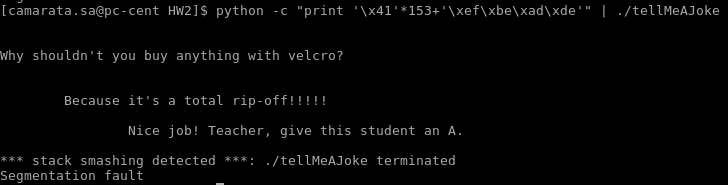
\includegraphics[scale=0.5]{./images/ss14.png}
\caption{Flag!}
\label{fig:Code}
\end{figure}

We've done it.  The flag has been captured!

\section{Part II: Extra Credit}

Rather than run through all the exact same steps that were completed in the assignment, this portion will focus more on the additional steps that were required to get to the flag. 

First we dump the strings to see if we can't identify what we are looking for.

\begin{figure}[H]
\centering
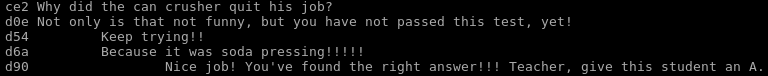
\includegraphics[scale=0.5]{./images/ss18.png}
\caption{strings}
\label{fig:Code}
\end{figure}

Then we disassemble the main() function.  This shows us that a function called handle\_connection() is called.

\begin{figure}[H]
\centering
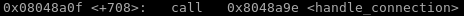
\includegraphics[scale=0.5]{./images/ss15.png}
\caption{disassemble main()}
\label{fig:Code}
\end{figure}

We disassemble the handle\_connection() function.  The only relevant thing we see here is that another function called work\_connection() is called.

\begin{figure}[H]
\centering
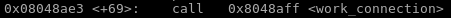
\includegraphics[scale=0.5]{./images/ss16.png}
\caption{disassemble handle\_connection()}
\label{fig:Code}
\end{figure}

In work connection we see that the programs is using the gets() call and we see that there are quite a few compares and jumps.  If we follow the same process as before, we can identify that 0xbas5eball leads us to the correct result.

\begin{figure}[H]
\centering
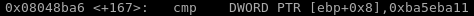
\includegraphics[scale=0.5]{./images/ss17.png}
\caption{disassemble work\_connection()}
\label{fig:Code}
\end{figure}

There are two major steps remaining and they are both dynamic analysis.  First discover how to manipulate the program.  Second identify the length of the buffer.  I figured that based on the name of the application 'serveMeAJoke' implied that we were running a server of some sort.  The most typical way to setup a server is to have a TCP socket bound to the system.  I ran 'netstat -anp | grep serve' to see if the process created a port binding.

\begin{figure}[H]
\centering
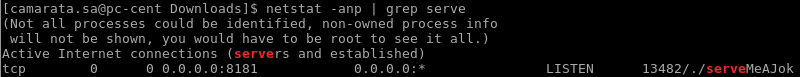
\includegraphics[scale=0.5]{./images/ss19.png}
\caption{netstat}
\label{fig:Code}
\end{figure}

As we can see above, the application is binding to port 8181.  The next step was to test an interaction with the server.  Here we use netcat to create a raw tcp connection to the socket.

\begin{figure}[H]
\centering
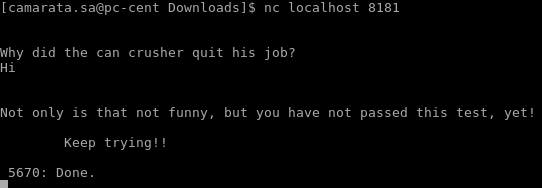
\includegraphics[scale=0.5]{./images/ss20.png}
\caption{netcat}
\label{fig:Code}
\end{figure}

Success.  We are prompted with a question upon connecting.  It accepted my input of 'Hi' and returned me a response that is obviously not the flag I am hoping for.

Once I started executing the program, I was having issues accessing the correct memory space.  I set an initial breakpoint after my first compare in the work\_connection() function, but I was failing to hit the break point.  Reading into the code further, I discovered that the program was calling a fork, implying that it was spawning another process for the handle\_connection() function.  A little research later, and I discovered that gdb has a mechanism for handling this.

\begin{figure}[H]
\centering
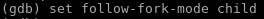
\includegraphics[scale=0.5]{./images/ss21.png}
\caption{fork}
\label{fig:Code}
\end{figure}

Now that I have instructed the debugger to follow the child process, I hit my break and I can review the stack and registers.

\begin{figure}[H]
\centering
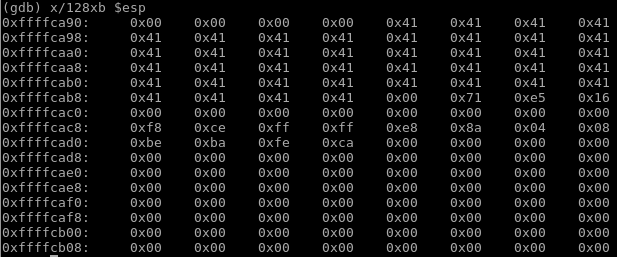
\includegraphics[scale=0.5]{./images/ss22.png}
\caption{stack}
\label{fig:Code}
\end{figure}

Here we see that my hex insert begins as 0xffffca94.

\begin{figure}[H]
\centering
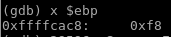
\includegraphics[scale=0.5]{./images/ss23.png}
\caption{ebp}
\label{fig:Code}
\end{figure}

Here we see that ebp is located at 0xffffcac8.  Simple hex math tells me that we are 0x34 hex or 52 decimal apart.  My compare is going to compare the hex value with what is contained at ebp + 8.  This means that we need to begin inserting  our attack 60 bytes into our input in little endian format.

\begin{figure}[H]
\centering
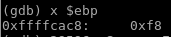
\includegraphics[scale=0.5]{./images/ss23.png}
\caption{attack}
\label{fig:Code}
\end{figure}

We run our attack and Voila.  We have successfully captured the flag!

\section{Conclusion}
In conclusion, I think this was an interesting exploitation project.  I would definitely be interested in a project that dives a bit deeper.  I felt that with the examples presented in class it was impossible to not be able to complete the steps needed to exploit these applications.  The extra credit did require a bit more knowledge about how to manipulate a linux system to get information about how the application is running, but I think the class should be capable of more complex disassembly.

\pagebreak
\begin{thebibliography}{9}
\bibitem{OSConcepts}
Abraham Silberschatz, Peter Baer Galvin, Greg Gagne
\textit{Operating System Concepts}
John Wiley \& Sons Inc. 2018
\end{thebibliography}
\end{document}